\documentclass[11pt,a4paper]{article}
\usepackage[utf8]{inputenc}
\usepackage[T1]{fontenc}
\usepackage{lmodern}
\usepackage[provide=*,spanish]{babel}
\usepackage[margin=2.2cm]{geometry}
\usepackage{booktabs,tabularx,array}
\usepackage{tikz}
\usetikzlibrary{positioning,arrows.meta}
\usepackage{listings}
\usepackage{xcolor}
\usepackage{enumitem}
\usepackage[hidelinks]{hyperref}

\setlist{itemsep=2pt,topsep=3pt}
\setlength{\parskip}{4pt}
\setlength{\parindent}{0pt}
\lstset{basicstyle=\ttfamily\small,columns=fixed,basewidth=0.5em,frame=single,
        framerule=0.3pt,rulecolor=\color{gray},backgroundcolor=\color{gray!6},
        xleftmargin=4pt,xrightmargin=4pt,aboveskip=6pt,belowskip=6pt}
\newcommand{\code}[1]{\texttt{#1}}
\newcommand{\menu}[1]{\textsf{\textbf{#1}}}
\newcolumntype{L}{>{\raggedright\arraybackslash}X}

\title{\textbf{Guía de uso del procesador ERV26}\\[2pt]
\large Proyecto \code{risvV\_E5} --- 25.30 Electrónica V (ITBA)}
\author{Matías}
\date{Noviembre 2026}

\begin{document}
\maketitle
\tableofcontents

\section{Qué es y qué contiene}

ERV26 es un procesador RISC-V (RV32I) con pipeline de 5 etapas, hecho con diagramas de bloques de Quartus para la placa DE10-Nano. La placa ejecuta programas escritos en C, muestra imagen por HDMI y lee botones conectados al GPIO. La explicación del diseño está en \code{doc/informe.pdf}.

El proyecto está en \code{C:\textbackslash Users\textbackslash matia\textbackslash Desktop\textbackslash risvV\_E5}:

\begin{center}
\begin{tabularx}{\linewidth}{lL}
\toprule
Carpeta / archivo & Contenido \\
\midrule
\code{risvV\_E5.qpf} & Proyecto de Quartus. \\
\code{risvV\_E5.bdf} & Diagrama de bloques de la placa (top). \\
\code{rtl/} & Bloques en Verilog y el núcleo \code{erv26\_core.bdf}. \\
\code{sw/} & Programas: \code{sw/demo/leds.c}, \code{sw/games/invaders/}, tests y \code{build.py}. \\
\code{programas/} & Programas ya compilados: \code{leds} e \code{invaders}. \\
\code{imem.hex}, \code{dmem\_b0..3.hex} & Programa que se carga en la placa al compilar en Quartus. \\
\code{cambiar\_programa.bat} & Copia uno de los programas compilados a la raíz. \\
\code{output\_files/risvV\_E5.sof} & Archivo para grabar la FPGA. \\
\code{clase/} & Simulaciones con ondas (GTKWave en WSL y ModelSim). \\
\code{electro5\_instalar/} & Instalador del entorno de simulación en WSL. \\
\code{doc/} & Informe técnico y esta guía. \\
\bottomrule
\end{tabularx}
\end{center}

\textbf{Programas incluidos:}
\begin{itemize}
\item \textbf{leds}: patrones en los LEDs que se eligen con los switches.
\item \textbf{invaders}: juego tipo \emph{Space Invaders} por HDMI, con botones en el GPIO. Es el que trae cargado el \code{.sof}.
\end{itemize}

\section{Herramientas necesarias}

\begin{center}
\begin{tabularx}{\linewidth}{lL}
\toprule
Herramienta & Para qué \\
\midrule
Quartus Prime 25.1 Lite, con soporte de Cyclone V & Compilar el hardware y grabar la placa. \\
Driver USB-Blaster II & Grabar la placa por USB (viene con Quartus). \\
WSL con Ubuntu & Compilar programas en C y correr las simulaciones (sección~\ref{sec:wslinst}). \\
gcc de RISC-V, Python 3, Icarus, GTKWave & Se instalan en WSL con el instalador (sección~\ref{sec:wsl}). \\
ModelSim 20.1 Starter (opcional) & Simular con la interfaz de ModelSim. \\
Placa DE10-Nano, fuente de 5\,V y cable mini-USB & Correr el procesador. \\
\bottomrule
\end{tabularx}
\end{center}

\subsection{Instalar WSL (una sola vez)}\label{sec:wslinst}

WSL permite usar Ubuntu dentro de Windows. Si ya está instalado (aparece \emph{Ubuntu} en el menú Inicio), pasar a la sección~\ref{sec:wsl}.

\begin{enumerate}
\item Abrir \textbf{PowerShell como administrador}: clic derecho en el botón Inicio $\to$ \menu{Terminal (Administrador)}.
\item Escribir:
\begin{lstlisting}
wsl --install
\end{lstlisting}
Instala WSL y Ubuntu. Tarda unos minutos.
\item \textbf{Reiniciar} la PC.
\item Abrir \textbf{Ubuntu} desde el menú Inicio. La primera vez pide crear un \textbf{usuario} y una \textbf{clave}. Anotar la clave: se usa para instalar programas (\code{sudo}).
\item Para comprobar, en PowerShell:
\begin{lstlisting}
wsl --list --verbose
\end{lstlisting}
Tiene que aparecer \code{Ubuntu} con \code{VERSION 2}.
\end{enumerate}

Notas:
\begin{itemize}
\item Si \code{wsl --install} muestra la ayuda en lugar de instalar, WSL ya estaba y falta Ubuntu: \code{wsl --install -d Ubuntu}.
\item Si da un error de virtualización (por ejemplo \code{0x80370102}), hay que activar la virtualización (\emph{Intel VT-x} / \emph{AMD-V}) en el BIOS de la PC.
\item En Windows 11, WSL ya muestra ventanas gráficas, así que GTKWave se abre como cualquier programa.
\item Desde Ubuntu, el disco \code{C:} de Windows está en \code{/mnt/c}. Por ejemplo, el proyecto está en:\\ \code{/mnt/c/Users/matia/Desktop/risvV\_E5}
\item Si te olvidaste la clave de Ubuntu, se cambia desde PowerShell con:\\ \code{wsl -u root passwd TU\_USUARIO}
\end{itemize}

\subsection{Instalar el entorno del proyecto (una sola vez)}\label{sec:wsl}

En la terminal de Ubuntu:
\begin{lstlisting}
cd ~
bash /mnt/c/Users/matia/Desktop/risvV_E5/electro5_instalar/instalar.sh
\end{lstlisting}
El instalador:
\begin{enumerate}
\item Borra \code{\textasciitilde/electro5}, pidiendo confirmación.
\item Copia ahí el entorno de simulación.
\item Instala con \code{apt} las herramientas que falten (gcc de RISC-V, Python, Icarus Verilog, GTKWave). Pide la clave de Ubuntu; al escribirla no se ve nada en pantalla.
\end{enumerate}
Al final tiene que decir \textbf{OK} en todas las herramientas.

\section{Flujo completo}

\begin{center}
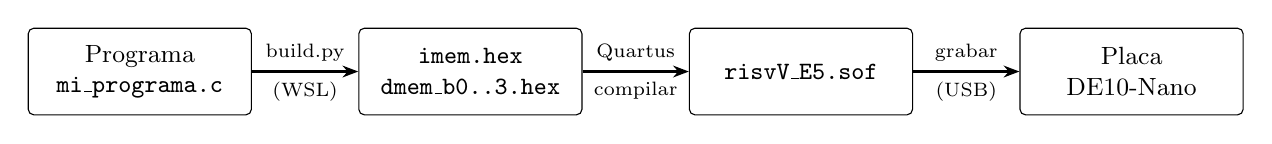
\begin{tikzpicture}[
  b/.style={draw,rounded corners=2pt,align=center,font=\small,minimum height=1.1cm,text width=2.6cm},
  a/.style={-{Stealth[length=2mm]},thick}]
\node[b] (c) {Programa\\ \code{mi\_programa.c}};
\node[b,right=1.35cm of c] (h) {\code{imem.hex}\\ \code{dmem\_b0..3.hex}};
\node[b,right=1.35cm of h] (s) {\code{risvV\_E5.sof}};
\node[b,right=1.35cm of s] (p) {Placa\\ DE10-Nano};
\draw[a] (c) -- node[above,font=\scriptsize]{build.py} node[below,font=\scriptsize]{(WSL)} (h);
\draw[a] (h) -- node[above,font=\scriptsize]{Quartus} node[below,font=\scriptsize]{compilar} (s);
\draw[a] (s) -- node[above,font=\scriptsize]{grabar} node[below,font=\scriptsize]{(USB)} (p);
\end{tikzpicture}
\end{center}

El programa no se carga por separado: queda \textbf{dentro del \code{.sof}}, como contenido inicial de las memorias de la FPGA. Por eso, cada vez que se cambia el programa hay que recompilar en Quartus y volver a grabar la placa.

\section{Escribir un programa}

Los programas se escriben en C, sin sistema operativo. Para usar los LEDs, switches, botones y video se incluye \code{erv26.h}:

\noindent\begin{minipage}{\linewidth}
\begin{lstlisting}[language=C]
#include "erv26.h"

int main(void) {
    for (;;)
        LEDS = SWITCHES;       /* los LEDs copian los switches */
}
\end{lstlisting}
\end{minipage}

\begin{center}
\begin{tabular}{lll}
\toprule
Nombre en C & Dirección & Uso \\
\midrule
\code{LEDS} & \code{0x80000000} & escribir: prende los 8 LEDs \\
\code{SWITCHES} & \code{0x80000004} & leer: los 4 switches \\
\code{CYCLES} & \code{0x80000008} & leer: ciclos de reloj desde el reset (50\,MHz) \\
\code{BUTTONS} & \code{0x8000000C} & leer: botones del GPIO (1 = apretado) \\
\code{FRAMES} & \code{0x80000010} & leer: cuadros de video (sube 60 veces por segundo) \\
\code{VIDEO\_CTRL} & \code{0x80000014} & escribir: página de video que se muestra \\
\code{FB\_PAGE(p)} & \code{0x40000000} & pantalla: 320$\times$240 píxeles, 1 byte por píxel \\
\bottomrule
\end{tabular}
\end{center}

Límites: 16\,KB de programa y 16\,KB de datos (variables y pila). No hay multiplicación en hardware: \code{*}, \code{/} y \code{\%} funcionan, pero más lentos.

\section{Compilar el programa}

\subsection{Opción A: usar un programa ya compilado}

En la carpeta del proyecto, desde una terminal de Windows (\code{cmd}):
\begin{lstlisting}
cambiar_programa.bat leds
cambiar_programa.bat invaders
\end{lstlisting}
Copia los \code{.hex} del programa elegido a la raíz del proyecto.

\subsection{Opción B: compilar un programa propio}

En la terminal de Ubuntu (WSL):
\begin{lstlisting}
cd /mnt/c/Users/matia/Desktop/risvV_E5
python3 sw/build.py mi_programa.c
\end{lstlisting}
Si el programa usa archivos de otra carpeta, se agrega con \code{-I}, por ejemplo:
\begin{lstlisting}
python3 sw/build.py sw/games/invaders/invaders.c -I sw/games/invaders
\end{lstlisting}

\code{build.py} deja en la raíz del proyecto:

\begin{center}
\begin{tabular}{ll}
\toprule
Archivo & Contenido \\
\midrule
\code{imem.hex} & instrucciones (memoria de programa) \\
\code{dmem\_b0..3.hex} & variables iniciales (memoria de datos, un archivo por byte) \\
\code{prog.lst} & listado en assembler, para revisar \\
\bottomrule
\end{tabular}
\end{center}

\section{Compilar en Quartus}

\begin{enumerate}
\item Abrir Quartus y \menu{File $\to$ Open Project} $\to$ \code{risvV\_E5.qpf}.
\item \menu{Processing $\to$ Start Compilation} (o el botón de \emph{play} azul de la barra). Tarda entre 8 y 12 minutos.
\item Al terminar, en \menu{Compilation Report}:
  \begin{itemize}
  \item \menu{Flow Summary}: tiene que decir \emph{Successful}. Ahí están los recursos usados (ALMs, memoria).
  \item \menu{Timing Analyzer $\to$ Summary}: el \emph{slack} de setup y de hold tiene que ser positivo (hoy: +4,6\,ns y +0,12\,ns).
  \end{itemize}
\item El resultado queda en \code{output\_files/risvV\_E5.sof}.
\end{enumerate}

Los avisos amarillos (\emph{warnings}) de memoria y de procesadores son normales.

\section{Grabar la placa}

\subsection{Conectar}\label{sec:driver}
\begin{enumerate}
\item Enchufar la \textbf{fuente de 5\,V} de la placa. El USB no la alimenta.
\item Conectar el mini-USB marcado \textbf{USB Blaster II} a la PC.
\end{enumerate}

La primera vez hay que instalar el driver:
\begin{enumerate}
\item Abrir el \menu{Administrador de dispositivos}.
\item Clic derecho sobre el dispositivo desconocido $\to$ \menu{Actualizar controlador} $\to$ \menu{Buscar en mi equipo}.
\item Elegir la carpeta \code{C:\textbackslash altera\_lite\textbackslash 25.1std\textbackslash quartus\textbackslash drivers}, con \menu{Incluir subcarpetas}.
\item Si aparece un segundo dispositivo desconocido, repetir.
\end{enumerate}

\subsection{Programar}
\begin{enumerate}
\item En Quartus: \menu{Tools $\to$ Programmer}.
\item \menu{Hardware Setup} $\to$ elegir \textbf{DE-SoC [USB-1]} $\to$ \menu{Close}. Modo: \textbf{JTAG}.
\item \menu{Auto Detect}. Si pregunta el dispositivo, elegir \textbf{5CSEBA6}. Si pregunta si actualiza la lista, \textbf{Yes}.
\item Aparecen dos filas. La primera es el procesador ARM de la placa y no se toca. Seleccionar la segunda, \textbf{5CSEBA6U23}.
\item \menu{Change File} $\to$ \code{output\_files/risvV\_E5.sof}.
\item Tildar solo \textbf{Program/Configure} en esa fila.
\item \menu{Start}. La barra tiene que llegar a \textbf{100\,\% (Successful)}.
\item Opcional: \menu{File $\to$ Save} guarda esta configuración (\code{risvV\_E5.cdf}) para la próxima vez.
\end{enumerate}

\textbf{Importante:} la FPGA se borra al apagar la placa. Cada vez que se prende hay que volver a apretar \menu{Start} en el Programmer.

\section{Usar la placa}

\begin{center}
\begin{tabular}{ll}
\toprule
Control & Función \\
\midrule
\code{KEY[0]} & Reset: reinicia el programa \\
\code{KEY[1]} (mantener) & Pausa el procesador \\
\code{SW[1:0]} (demo de LEDs) & Patrón: contador, auto fantástico, llenado, Fibonacci \\
\code{SW[2]} (demo de LEDs) & Velocidad lenta o rápida \\
\code{SW[3]} (demo de LEDs) & Pausa la animación \\
\bottomrule
\end{tabular}
\end{center}

\subsection{Juego por HDMI}

Conectar un monitor al HDMI de la placa. La imagen aparece alrededor de 1 segundo después del reset. Los botones van en el header \textbf{GPIO 0 (JP1)}, cada uno entre su pin y GND, sin resistencias:

\begin{center}
\begin{tabular}{cl}
\toprule
Pin de JP1 & Función \\
\midrule
1 & Izquierda \\
2 & Derecha \\
3 & Disparo \\
4 & Start \\
12 o 30 & GND (común de los botones) \\
\bottomrule
\end{tabular}
\end{center}

Los pines de la FPGA son de \textbf{3,3\,V}. No conectar nada al pin 11 (5\,V) ni llevar señales de 5\,V a los GPIO.

\section{Probar en simulación (opcional)}

\subsection{En WSL}
\begin{lstlisting}
cd ~/electro5
make                # menu de opciones
make tests          # verifica el procesador contra el modelo de referencia
make pipeline       # ondas del pipeline en GTKWave
make test T=rv32ui-beq
make placa          # placa completa con la demo de LEDs
make video          # salida HDMI y cuadros en PNG
make juego          # cuadros del juego en PNG (unos minutos)
\end{lstlisting}

\subsection{En ModelSim}
\begin{enumerate}
\item \menu{File $\to$ Change Directory} $\to$ \code{risvV\_E5\textbackslash clase\textbackslash modelsim}.
\item En el \menu{Transcript}, escribir por ejemplo:
\begin{lstlisting}
do pipeline.do
do test.do rv32ui-beq
do regresion.do
do placa.do
\end{lstlisting}
\end{enumerate}

Más detalle en \code{clase/LEEME.md} y \code{clase/modelsim/LEEME.md}.

\section{Problemas comunes}

\begin{center}
\begin{tabularx}{\linewidth}{lL}
\toprule
Problema & Qué hacer \\
\midrule
Windows no detecta la placa & Revisar la fuente de 5\,V (LED de power prendido) y probar otro cable o puerto USB. \\
\emph{No hardware} en el Programmer & Instalar el driver del USB-Blaster II (sección~\ref{sec:driver}). \\
El Programmer falla al grabar & Verificar que el \code{.sof} esté en la fila \textbf{5CSEBA6U23} y no en la del ARM. \\
Pantalla negra & Esperar 1 segundo o apretar \code{KEY[0]}. Revisar el cable HDMI. \\
Cambié el programa y no se nota & Recompilar en Quartus y volver a grabar la placa. \\
\code{build.py} no encuentra el compilador & Correr el instalador de WSL (sección~\ref{sec:wsl}). \\
\bottomrule
\end{tabularx}
\end{center}

\end{document}
